% Created by tikzDevice version 0.8.1 on 2015-11-21 14:38:50
% !TEX encoding = UTF-8 Unicode
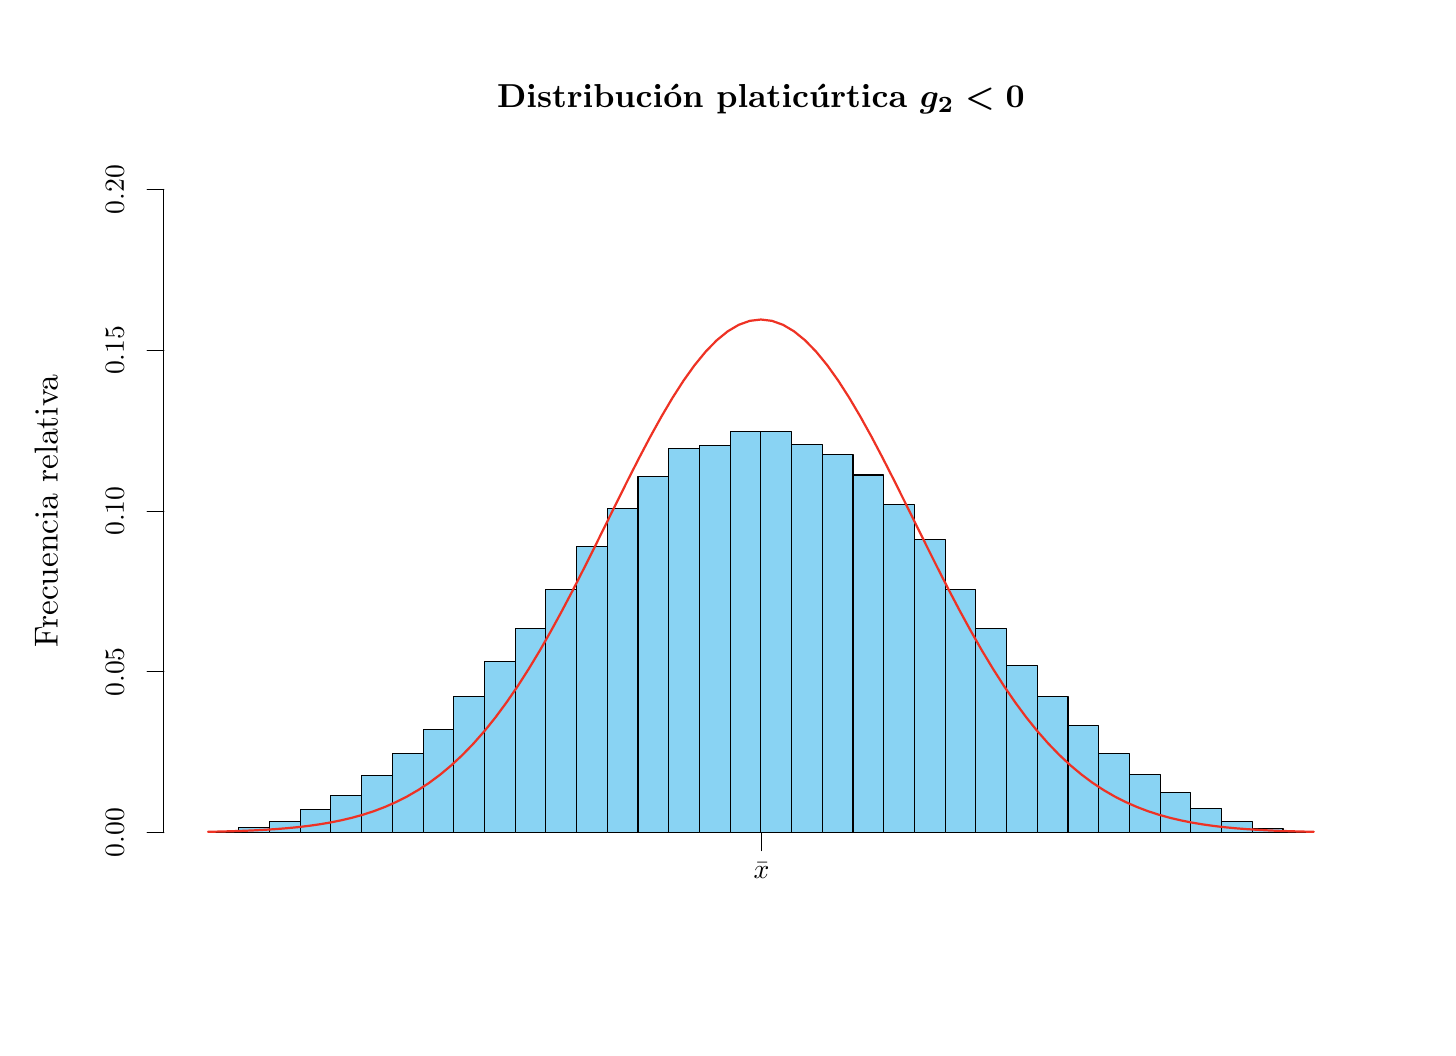
\begin{tikzpicture}[x=1pt,y=1pt]
\definecolor{fillColor}{RGB}{255,255,255}
\path[use as bounding box,fill=fillColor,fill opacity=0.00] (0,0) rectangle (505.89,361.35);
\begin{scope}
\path[clip] (  0.00,  0.00) rectangle (505.89,361.35);
\definecolor{drawColor}{RGB}{0,0,0}

\node[text=drawColor,anchor=base,inner sep=0pt, outer sep=0pt, scale=  1.20, font=\boldmath] at (264.94,332.61)
{\bfseries Distribución platicúrtica $g_2<0$};

\node[text=drawColor,rotate= 90.00,anchor=base,inner sep=0pt, outer sep=0pt, scale=  1.20] at ( 10.80,186.67)
{Frecuencia relativa};
\end{scope}
\begin{scope}
\path[clip] ( 49.20, 61.20) rectangle (480.69,312.15);
\definecolor{drawColor}{RGB}{0,0,0}
\definecolor{fillColor}{RGB}{137,211,243}

\path[draw=drawColor,line width= 0.4pt,line join=round,line cap=round,fill=fillColor] ( 65.18, 70.49) rectangle ( 76.28, 70.66);

\path[draw=drawColor,line width= 0.4pt,line join=round,line cap=round,fill=fillColor] ( 76.28, 70.49) rectangle ( 87.38, 72.27);

\path[draw=drawColor,line width= 0.4pt,line join=round,line cap=round,fill=fillColor] ( 87.38, 70.49) rectangle ( 98.48, 74.36);

\path[draw=drawColor,line width= 0.4pt,line join=round,line cap=round,fill=fillColor] ( 98.48, 70.49) rectangle (109.57, 78.85);

\path[draw=drawColor,line width= 0.4pt,line join=round,line cap=round,fill=fillColor] (109.57, 70.49) rectangle (120.67, 84.04);

\path[draw=drawColor,line width= 0.4pt,line join=round,line cap=round,fill=fillColor] (120.67, 70.49) rectangle (131.77, 91.10);

\path[draw=drawColor,line width= 0.4pt,line join=round,line cap=round,fill=fillColor] (131.77, 70.49) rectangle (142.87, 98.97);

\path[draw=drawColor,line width= 0.4pt,line join=round,line cap=round,fill=fillColor] (142.87, 70.49) rectangle (153.97,107.87);

\path[draw=drawColor,line width= 0.4pt,line join=round,line cap=round,fill=fillColor] (153.97, 70.49) rectangle (165.06,119.51);

\path[draw=drawColor,line width= 0.4pt,line join=round,line cap=round,fill=fillColor] (165.06, 70.49) rectangle (176.16,132.20);

\path[draw=drawColor,line width= 0.4pt,line join=round,line cap=round,fill=fillColor] (176.16, 70.49) rectangle (187.26,144.35);

\path[draw=drawColor,line width= 0.4pt,line join=round,line cap=round,fill=fillColor] (187.26, 70.49) rectangle (198.36,158.29);

\path[draw=drawColor,line width= 0.4pt,line join=round,line cap=round,fill=fillColor] (198.36, 70.49) rectangle (209.46,173.78);

\path[draw=drawColor,line width= 0.4pt,line join=round,line cap=round,fill=fillColor] (209.46, 70.49) rectangle (220.55,187.44);

\path[draw=drawColor,line width= 0.4pt,line join=round,line cap=round,fill=fillColor] (220.55, 70.49) rectangle (231.65,199.20);

\path[draw=drawColor,line width= 0.4pt,line join=round,line cap=round,fill=fillColor] (231.65, 70.49) rectangle (242.75,209.17);

\path[draw=drawColor,line width= 0.4pt,line join=round,line cap=round,fill=fillColor] (242.75, 70.49) rectangle (253.85,210.52);

\path[draw=drawColor,line width= 0.4pt,line join=round,line cap=round,fill=fillColor] (253.85, 70.49) rectangle (264.94,215.44);

\path[draw=drawColor,line width= 0.4pt,line join=round,line cap=round,fill=fillColor] (264.94, 70.49) rectangle (276.04,215.27);

\path[draw=drawColor,line width= 0.4pt,line join=round,line cap=round,fill=fillColor] (276.04, 70.49) rectangle (287.14,210.88);

\path[draw=drawColor,line width= 0.4pt,line join=round,line cap=round,fill=fillColor] (287.14, 70.49) rectangle (298.24,207.17);

\path[draw=drawColor,line width= 0.4pt,line join=round,line cap=round,fill=fillColor] (298.24, 70.49) rectangle (309.34,199.69);

\path[draw=drawColor,line width= 0.4pt,line join=round,line cap=round,fill=fillColor] (309.34, 70.49) rectangle (320.43,189.01);

\path[draw=drawColor,line width= 0.4pt,line join=round,line cap=round,fill=fillColor] (320.43, 70.49) rectangle (331.53,176.45);

\path[draw=drawColor,line width= 0.4pt,line join=round,line cap=round,fill=fillColor] (331.53, 70.49) rectangle (342.63,158.49);

\path[draw=drawColor,line width= 0.4pt,line join=round,line cap=round,fill=fillColor] (342.63, 70.49) rectangle (353.73,144.25);

\path[draw=drawColor,line width= 0.4pt,line join=round,line cap=round,fill=fillColor] (353.73, 70.49) rectangle (364.83,130.90);

\path[draw=drawColor,line width= 0.4pt,line join=round,line cap=round,fill=fillColor] (364.83, 70.49) rectangle (375.92,119.81);

\path[draw=drawColor,line width= 0.4pt,line join=round,line cap=round,fill=fillColor] (375.92, 70.49) rectangle (387.02,109.10);

\path[draw=drawColor,line width= 0.4pt,line join=round,line cap=round,fill=fillColor] (387.02, 70.49) rectangle (398.12, 99.14);

\path[draw=drawColor,line width= 0.4pt,line join=round,line cap=round,fill=fillColor] (398.12, 70.49) rectangle (409.22, 91.48);

\path[draw=drawColor,line width= 0.4pt,line join=round,line cap=round,fill=fillColor] (409.22, 70.49) rectangle (420.32, 85.12);

\path[draw=drawColor,line width= 0.4pt,line join=round,line cap=round,fill=fillColor] (420.32, 70.49) rectangle (431.41, 79.24);

\path[draw=drawColor,line width= 0.4pt,line join=round,line cap=round,fill=fillColor] (431.41, 70.49) rectangle (442.51, 74.57);

\path[draw=drawColor,line width= 0.4pt,line join=round,line cap=round,fill=fillColor] (442.51, 70.49) rectangle (453.61, 72.07);

\path[draw=drawColor,line width= 0.4pt,line join=round,line cap=round,fill=fillColor] (453.61, 70.49) rectangle (464.71, 70.75);
\end{scope}
\begin{scope}
\path[clip] (  0.00,  0.00) rectangle (505.89,361.35);
\definecolor{drawColor}{RGB}{0,0,0}

\path[draw=drawColor,line width= 0.4pt,line join=round,line cap=round] (265.20, 70.49) -- (265.20, 64);

\node[text=drawColor,anchor=base,inner sep=0pt, outer sep=0pt, scale=  1.00] at (265.20, 54) {$\bar x$};

\path[draw=drawColor,line width= 0.4pt,line join=round,line cap=round] ( 49.20, 70.49) -- ( 49.20,302.86);

\path[draw=drawColor,line width= 0.4pt,line join=round,line cap=round] ( 49.20, 70.49) -- ( 43.20, 70.49);

\path[draw=drawColor,line width= 0.4pt,line join=round,line cap=round] ( 49.20,128.58) -- ( 43.20,128.58);

\path[draw=drawColor,line width= 0.4pt,line join=round,line cap=round] ( 49.20,186.67) -- ( 43.20,186.67);

\path[draw=drawColor,line width= 0.4pt,line join=round,line cap=round] ( 49.20,244.77) -- ( 43.20,244.77);

\path[draw=drawColor,line width= 0.4pt,line join=round,line cap=round] ( 49.20,302.86) -- ( 43.20,302.86);

\node[text=drawColor,rotate= 90.00,anchor=base,inner sep=0pt, outer sep=0pt, scale=  1.00] at ( 34.80, 70.49) {0.00};

\node[text=drawColor,rotate= 90.00,anchor=base,inner sep=0pt, outer sep=0pt, scale=  1.00] at ( 34.80,128.58) {0.05};

\node[text=drawColor,rotate= 90.00,anchor=base,inner sep=0pt, outer sep=0pt, scale=  1.00] at ( 34.80,186.67) {0.10};

\node[text=drawColor,rotate= 90.00,anchor=base,inner sep=0pt, outer sep=0pt, scale=  1.00] at ( 34.80,244.77) {0.15};

\node[text=drawColor,rotate= 90.00,anchor=base,inner sep=0pt, outer sep=0pt, scale=  1.00] at ( 34.80,302.86) {0.20};
\end{scope}
\begin{scope}
\path[clip] ( 49.20, 61.20) rectangle (480.69,312.15);
\definecolor{drawColor}{RGB}{238,50,36}

\path[draw=drawColor,line width= 0.8pt,line join=round,line cap=round] ( 65.18, 70.78) --
	( 69.18, 70.86) --
	( 73.17, 70.97) --
	( 77.17, 71.10) --
	( 81.16, 71.26) --
	( 85.16, 71.47) --
	( 89.15, 71.72) --
	( 93.15, 72.03) --
	( 97.14, 72.41) --
	(101.14, 72.87) --
	(105.13, 73.43) --
	(109.13, 74.09) --
	(113.12, 74.89) --
	(117.12, 75.83) --
	(121.11, 76.94) --
	(125.11, 78.24) --
	(129.11, 79.76) --
	(133.10, 81.52) --
	(137.10, 83.54) --
	(141.09, 85.85) --
	(145.09, 88.48) --
	(149.08, 91.45) --
	(153.08, 94.79) --
	(157.07, 98.51) --
	(161.07,102.64) --
	(165.06,107.18) --
	(169.06,112.15) --
	(173.05,117.55) --
	(177.05,123.37) --
	(181.04,129.61) --
	(185.04,136.23) --
	(189.03,143.23) --
	(193.03,150.55) --
	(197.03,158.15) --
	(201.02,165.98) --
	(205.02,173.97) --
	(209.01,182.04) --
	(213.01,190.13) --
	(217.00,198.14) --
	(221.00,205.98) --
	(224.99,213.56) --
	(228.99,220.78) --
	(232.98,227.55) --
	(236.98,233.78) --
	(240.97,239.37) --
	(244.97,244.26) --
	(248.96,248.36) --
	(252.96,251.62) --
	(256.95,253.98) --
	(260.95,255.41) --
	(264.94,255.89) --
	(268.94,255.41) --
	(272.94,253.98) --
	(276.93,251.62) --
	(280.93,248.36) --
	(284.92,244.26) --
	(288.92,239.37) --
	(292.91,233.78) --
	(296.91,227.55) --
	(300.90,220.78) --
	(304.90,213.56) --
	(308.89,205.98) --
	(312.89,198.14) --
	(316.88,190.13) --
	(320.88,182.04) --
	(324.87,173.97) --
	(328.87,165.98) --
	(332.86,158.15) --
	(336.86,150.55) --
	(340.86,143.23) --
	(344.85,136.23) --
	(348.85,129.61) --
	(352.84,123.37) --
	(356.84,117.55) --
	(360.83,112.15) --
	(364.83,107.18) --
	(368.82,102.64) --
	(372.82, 98.51) --
	(376.81, 94.79) --
	(380.81, 91.45) --
	(384.80, 88.48) --
	(388.80, 85.85) --
	(392.79, 83.54) --
	(396.79, 81.52) --
	(400.78, 79.76) --
	(404.78, 78.24) --
	(408.77, 76.94) --
	(412.77, 75.83) --
	(416.77, 74.89) --
	(420.76, 74.09) --
	(424.76, 73.43) --
	(428.75, 72.87) --
	(432.75, 72.41) --
	(436.74, 72.03) --
	(440.74, 71.72) --
	(444.73, 71.47) --
	(448.73, 71.26) --
	(452.72, 71.10) --
	(456.72, 70.97) --
	(460.71, 70.86) --
	(464.71, 70.78);
\end{scope}
\end{tikzpicture}
